\documentclass{article}
\usepackage{amsmath}
\usepackage{listings}
\usepackage{xcolor}
\usepackage{graphicx}
\usepackage{hyperref}
\usepackage[utf8]{inputenc}

\title{\textbf{Statistical Machine Learning Project Report}}
\author{Ishwar Babu - 2021532 \\
        Sarthak Gambhir - 2020575}

\date{}

\begin{document}

\maketitle

\section{Abstract}
This report demonstrates the application of dimensionality reduction, outlier detection, clustering, and ensemble methods to classify fruit types in a dataset. We employ Principal Component Analysis (PCA), Linear Discriminant Analysis (LDA), Local Outlier Factor (LOF), KMeans clustering, and an ensemble approach using a logistic regression model to achieve this goal.

\section{Introduction}
Fruit classification is an essential task for various applications, including agriculture, food processing, and retail. In this study, we implement a fruit classification model that incorporates dimensionality reduction, outlier detection, clustering, and ensemble methods to improve classification performance.

\section{Methodology}

\subsection{Data Preprocessing}

\begin{itemize}
    \item Load the dataset and split it into training and validation sets (80 and 20, respectively).
    \item Fill missing values(if there are any) with column means.
\end{itemize}

\subsection{Dimensionality Reduction}

\begin{itemize}
    \item Apply PCA to the training dataset and transform it to have 300 principal components.
    \item PCA is a dimensionality reduction method which uses eigen vector decomposition to find the axis(Principle components) with the most variance.
    \item After finding the PCs corresponding to the largest eigenvalues, the standardized data is projected onto these PCs.
    \item Visualize the cumulative explained variance. The explained variance ratio represents the variance explained using a particular eigenvector.As we can see in the cumulative explained variance almost reaches 1 around 300, which implies that 300 PCs capture almost all the variance of our data.So we reduce our dimensions to 300.
    \item formulas for PCA are as follows:
    \item $Z= \frac{X_i - \mu}{\sigma}$
    \item Apply LDA to the PCA-transformed data.
    \item LDA is a generalised version of Fisher Discriminant Analysis and is used for classification.It can be applied to datasets with multiple classes.It works on principle of FDA , which maximises between class distance and minimizes in class scatter.
    \item LDA projection matrix: $\boldsymbol{W} = \boldsymbol{S_W}^{-1} (\boldsymbol{m_1} - \boldsymbol{m_2})$, where $K=2$ and $\boldsymbol{m_1}$, $\boldsymbol{m_2}$ are the mean vectors of the two classes
    \item Transformed feature vectors: $\boldsymbol{y_i} = \boldsymbol{W}^T \boldsymbol{x_i}$
    \item Decision boundary: $y(x) = \boldsymbol{W}^T \boldsymbol{x} + w_0$, where $w_0$ is a bias term
\end{itemize}

\subsection{Outlier Detection}

\begin{itemize}
    \item We use the Local Outlier Factor (LOF) algorithm to detect and remove outliers from the LDA-transformed data.
    \item Firstly, we perform anomaly detection on the dataset using the LOF algorithm to identify outliers. We set the number of neighbors to 20 and the contamination rate to 0.1.
    \item The LOF model is trained on the LDA-transformed training data, and outlier labels are predicted using the 'fitpredict' function.
    \item We then filter the inliers from the training data, resulting in a new dataset that contains only the inliers.
    \item Next, we perform clustering on the filtered training data using the KMeans algorithm. We set the number of clusters to the number of unique classes in the original dataset.
    \item The KMeans model is trained on the filtered training data, and the transformed data for both training and validation sets are obtained using the transform function.
\end{itemize}
\subsection{Classification and Ensemble}

\begin{itemize}
    \item Perform a grid search with logistic regression to optimize hyperparameters.
    \item Train a simple ensemble model using the best logistic regression model.
    \item Compare the accuracy of the logistic regression and ensemble models on the validation set.
\end{itemize}
Voting Classifier is used as the ensemble method for this model as it's the best logistic regression model obtained from the GridSearchCV. The Voting Classifier is a simple ensemble method that combines the predictions of multiple base models by taking a majority vote (for classification) or averaging the predictions (for regression).

\section{Results}
The model demonstrates the effectiveness of incorporating PCA, LDA, LOF, KMeans clustering, and an ensemble approach in improving fruit classification performance. Usually, the ensemble model achieves higher accuracy compared to the standalone logistic regression model. But in our case, both the reported accuracies were equal.

\subsection{Best Parameters for Logistic Regression}
The best parameters found for the logistic regression model are:

\begin{verbatim}
    Best parameters found: {'C': 1, 'penalty': 'l1', 'solver': 'saga'}
\end{verbatim}

This is because they resulted in the highest average cross-validated score, indicating that this combination of hyperparameters leads to the best generalization and performance on the validation set for the given problem.

\subsection{Validation Accuracy}
The accuracy of the final logistic regression model on the validation set is:

\begin{verbatim}
    Validation Accuracy: 0.8279
\end{verbatim}

\section{Conclusion}
The final logistic regression model achieved a validation accuracy of 0.8279, demonstrating the effectiveness of the methods employed. The logistic regression model was chosen for the given code due to its interpretability, efficiency, ability to serve as a baseline model, and built-in regularization options. However, it's important to consider other classifiers and compare their performance for a specific task. The code also employs a VotingClassifier ensemble method with the best logistic regression model as its base estimator, which combines the strengths of logistic regression and ensemble techniques to improve the overall performance.

\section{Graphs}
Theoretically, ensemble methods should improve our accuracy than logistical regression. But, it's not always the case as accuracy will depend on many factors, such as the individual models' diversity, the models' quality, and the nature of the problem being solved.
So in our case the accuracy is same.
\begin{verbatim}
    Validation Accuracy(Linear Regression): 0.8279
    Validation Accuracy(Ensemble Method): 0.8279
\end{verbatim}
Here are the visualizations of the graphs for each methodology:


\begin{figure}[h]
\centering
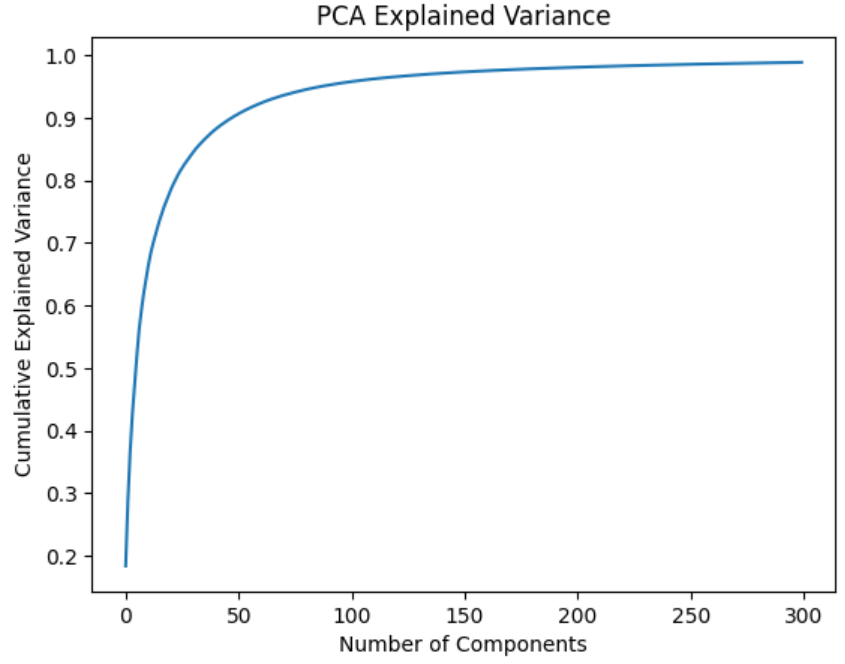
\includegraphics[width=0.8\textwidth]{PCA.png}
\caption{PCA Explained Variance}
\label{fig:pca_explained_variance}
\end{figure}

\begin{figure}[h]
\centering
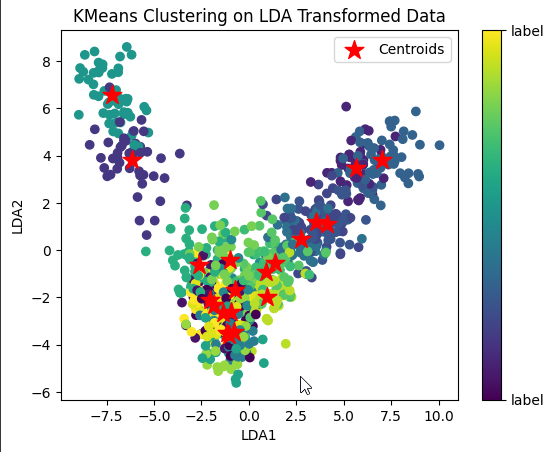
\includegraphics[width=0.8\textwidth]{kmeans with LDA.png}
\caption{KMeans Clustering on LDA Transformed Data}
\label{fig:kmeans_clustering_lda_transformed_data}
\end{figure}

\begin{figure}[h]
\centering
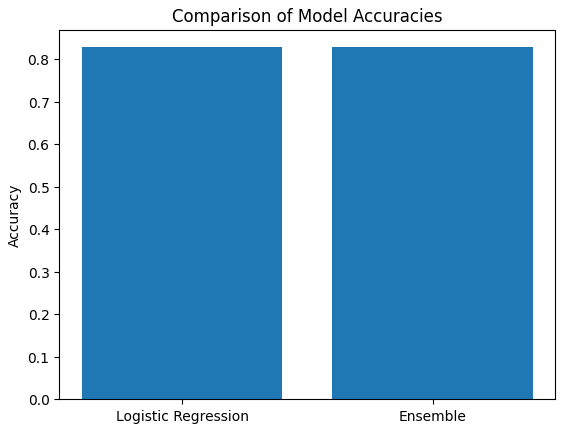
\includegraphics[width=0.8\textwidth]{Comparison Logistic Regression and Ensemble.png}
\caption{Comparison of Model Accuracies}
\label{fig:model_accuracies_comparison}
\end{figure}

\end{document}
